\section{Edit Menu}
The only option is Calibrate Spectrum. This will launch a new window, seen in Figure \ref{fig:calibrate_window}. The main widget features two indepenedent graphs. The upper represents the raw, uncalibrated spectrum and is plotted on a channel basis. The lower graph shows a linearly calibrated spectrum, this initializes to a 3MeV maximum, with a single peak added it adjusts to a 0 intercept with a single point slope, two or more calibration points results in a linear least squares regression fit being shown. The dotted black line that appears is used to track the cursor to help in the identification of peak centroids. Double-right clicking with initiate a input dialog that will take the energy of the peak in MeV. This will be added to the widget on the left-hand side. Double-left clicking will remove the peak-channel pair. There is no limit to the numer of peaks that can be selected, but a minimum of two are required. This window has one drop down in the menu bar: 
\begin{figure}[h!]
	\centering
	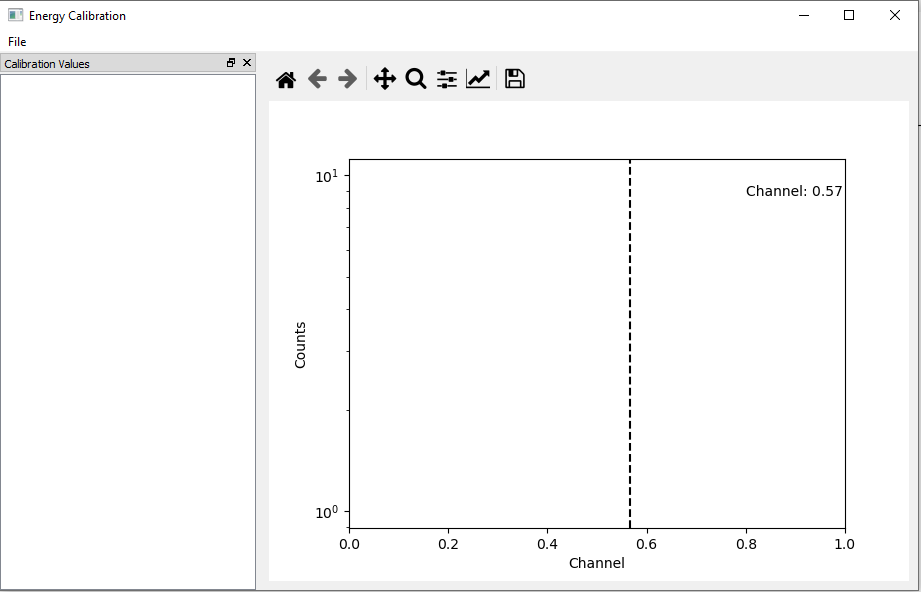
\includegraphics[width=\linewidth]{Calibrate.png}
	\caption{Calibration interface.}
	\label{fig:calibrate_window}
\end{figure}


	\subsection{Load New Spectrum}
		This will load the per channel counts in the spectrum. This will accept plain text, comma-seperated, and IAEA file types. It expects a single column of data for the plain text and comma-seperated variants.

	\subsection{Calibrate}
		This loads a drop down menu with the following options:
				\subsubsection{Linear}
				Performs a linear least squares regression, ultimately resulting in the calibration being in the form of:
				\begin{equation}
				 	y=mx+b
				\label{eq:linear}
				\end{equation}
				\subsubsection{Deviation Pairs}
				Conducts a linear least squares fit, the determines the devaition from this at the known points to create and scale each data point. This can be used to generate a non-linear calibration.
				\subsubsection{External Calibration}
				Used if a known slope and intercept are to be input. It will fit the calibration to equation \ref{eq:linear}.
				\subsubsection{Segmented Linear}
				Fits a line between each successive point of the inputs.
	\subsection{Save Calibration}
	Will save a single column of that relate the channel to calibrated energy as a plain text file(.txt) to the specified location.